\documentclass{article}
\usepackage{amsmath, sfmath, multicol, tkz-euclide, array, enumerate, tcolorbox, tabularray}
\renewcommand{\familydefault}{\sfdefault}
\setlength{\parindent}{0cm}
\pagestyle{empty}
\usepackage[left=1in, top=0.5in, right=1in, bottom=0.5in]{geometry}
\tikzset{>=stealth}
\tcbset{colback=white}

\newcounter{example}[section]
\newenvironment{example}[1][]{\refstepcounter{example}\par\medskip
   {\color{red}\textbf{Example~\theexample. #1}}}{\medskip}

\begin{document}

\section*{Dilations}

\begin{tcolorbox}[colframe=orange!70!white, coltitle=black, title=\textbf{Today I Can}]
\begin{enumerate}
    \item Perform dilations of figures.
\end{enumerate}
\end{tcolorbox}
\smallskip

\begin{tcolorbox}[colframe=black!20!white, opacitybacktitle=0.1, coltitle=black, title=\textbf{Dilations}]
A transformation to a figure that will produce a similar one that is either larger (an \emph{enlargement}) or smaller (a \emph{reduction}) than the original.
\end{tcolorbox}
\bigskip 

We use the scale to determine what we multiply the sides by.
\begin{itemize}
    \item If the scale is larger than 1, the dilation is an enlargement.
    \item If the scale is between 0 and 1, the dilation is a reduction.
\end{itemize}
\bigskip 

When dilating figures in the coordinate plane, multiply the coordinates of the vertices by the scale. \newline\\

\begin{example}
Find the coordinates of $\triangle G'P'Z'$ after each dilation. Then graph the result.


\begin{enumerate}[(a)]
\begin{multicols}{2}
    \item Scale factor of 2 \newline 
    
    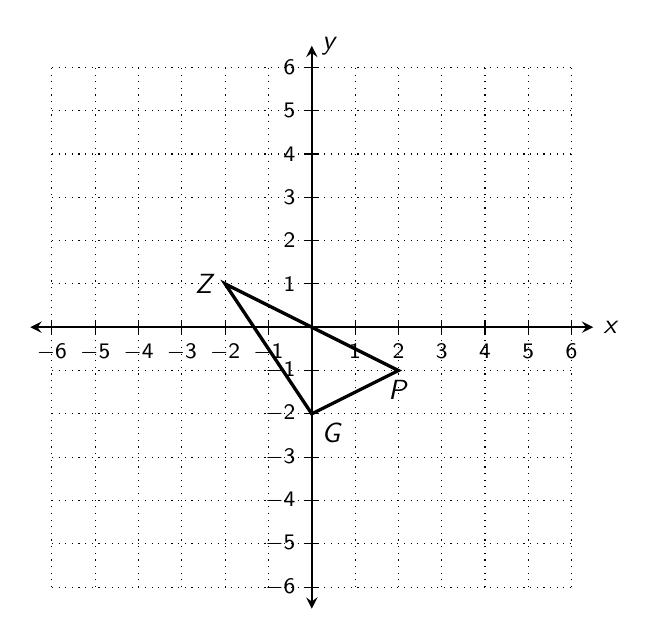
\begin{tikzpicture}[scale=0.55]
    \draw[<->, thick] (-6.5,0) -- (6.5,0) node [right] {$x$};
    \draw[<->, thick] (0,-6.5) -- (0,6.5) node [right] {$y$};
    \draw[dotted] (-6,-6) grid (6,6);
    \foreach \x in {-6,...,-1,,1,...,6}
    \draw (\x, 0.15) -- (\x,-0.15) node [below] {\footnotesize$\x$};
    \foreach \y in {-6,...,-1,,1,...,6}
    \draw (0.15,\y) -- (-0.15,\y) node [left] {\footnotesize $\y$};
    \coordinate (G) at (0,-2);
    \coordinate (P) at (2,-1);
    \coordinate (Z) at (-2,1);
    \node at (G) [anchor = north west] {$G$};
    \node at (P) [anchor = north] {$P$};
    \node at (Z) [anchor = east] {$Z$};
    \draw[very thick] (G) -- (P) -- (Z) --  cycle;
    \end{tikzpicture}

    \item Scale factor of $\frac{1}{2}$ \newline 
    
    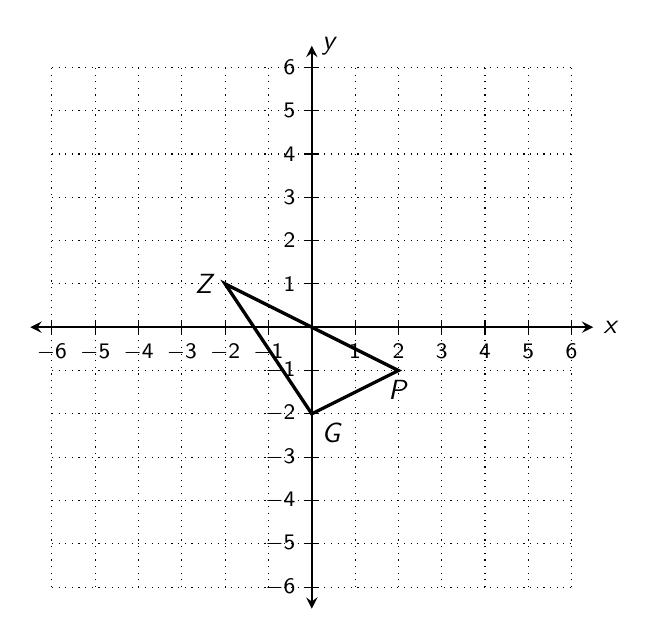
\begin{tikzpicture}[scale=0.55]
    \draw[<->, thick] (-6.5,0) -- (6.5,0) node [right] {$x$};
    \draw[<->, thick] (0,-6.5) -- (0,6.5) node [right] {$y$};
    \draw[dotted] (-6,-6) grid (6,6);
    \foreach \x in {-6,...,-1,,1,...,6}
    \draw (\x, 0.15) -- (\x,-0.15) node [below] {\footnotesize$\x$};
    \foreach \y in {-6,...,-1,,1,...,6}
    \draw (0.15,\y) -- (-0.15,\y) node [left] {\footnotesize $\y$};
    \coordinate (G) at (0,-2);
    \coordinate (P) at (2,-1);
    \coordinate (Z) at (-2,1);
    \node at (G) [anchor = north west] {$G$};
    \node at (P) [anchor = north] {$P$};
    \node at (Z) [anchor = east] {$Z$};
    \draw[very thick] (G) -- (P) -- (Z) --  cycle;
    \end{tikzpicture}
    \end{multicols}

    \newpage 

    \item Scale factor of 1.5 \label{1c} \newline 

    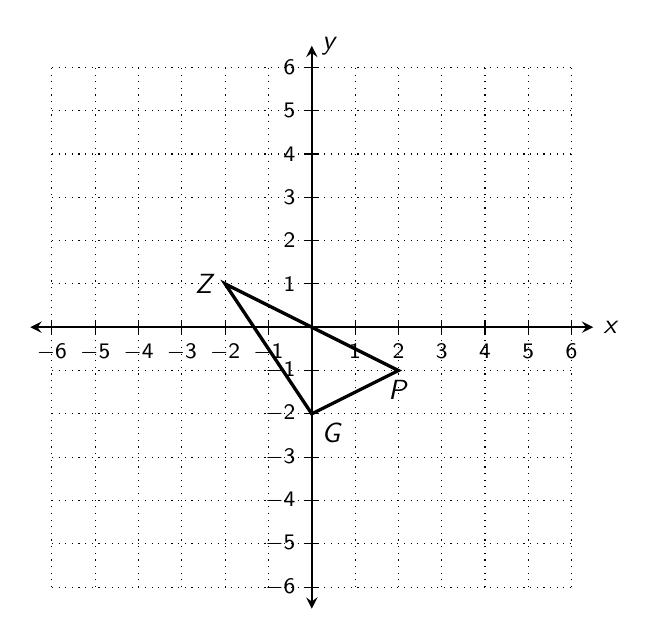
\begin{tikzpicture}[scale=0.55]
    \draw[<->, thick] (-6.5,0) -- (6.5,0) node [right] {$x$};
    \draw[<->, thick] (0,-6.5) -- (0,6.5) node [right] {$y$};
    \draw[dotted] (-6,-6) grid (6,6);
    \foreach \x in {-6,...,-1,,1,...,6}
    \draw (\x, 0.15) -- (\x,-0.15) node [below] {\footnotesize$\x$};
    \foreach \y in {-6,...,-1,,1,...,6}
    \draw (0.15,\y) -- (-0.15,\y) node [left] {\footnotesize $\y$};
    \coordinate (G) at (0,-2);
    \coordinate (P) at (2,-1);
    \coordinate (Z) at (-2,1);
    \node at (G) [anchor = north west] {$G$};
    \node at (P) [anchor = north] {$P$};
    \node at (Z) [anchor = east] {$Z$};
    \draw[very thick] (G) -- (P) -- (Z) --  cycle;
    \end{tikzpicture}
\end{enumerate}
\end{example}

\vspace{1in}

\begin{example}
Calculate the slope of $\overline{PG}$ from Example 1\ref{1c}. Then calculate the slope of $\overline{P'G'}$. \newline\\ What do you notice?
\end{example}

\end{document}
